


\documentclass[main.tex]{subfiles}

\begin{document}


\chapter{Crack propagation}
\label{LEC:CrackPropagation}

In the previous lecture, we have analyzed the correspondence between the fracture and damage using a uni-axial example. In the present lecture we apply the same concepts to a two-dimensional case of stable crack propagation.
In particular, we are going to use the three-point bending test as a means of  rendering an elementary crack-propagation scenario, namely a stable crack running along a predefined straight path. After discussing the test setup, we provide the test results in terms of load-deflection curve. Then, we will construct a numerical model that can reproduce such a behavior, specify the required material parameters and how to identify them.
Similarly to the previous lecture, we will consider the link between fracture and damage concepts that are both included in any finite element computation involving strain-softening material behavior

\section{Propagation of a straight crack}

\mnote{Why notched three-point bending test?}
An isolated tensile crack, mode-I crack, can be initiated using a notched specimen. The most common configurations used to study the cracking behavior for a tensile crack denoted as mode I are the wedge splitting test and notched, three-point bending test. Both these tests aim at the characterization of the material behavior in terms of the softening law describing the relation between the tensile stress transmitted across the localization zone and the corresponding crack opening. 

Due to its simplicity, three-point-bending test on a notched concrete has become a standard (RILEM) to determine the fracture energy $G_\mathrm{F}$ characterizing the cracking behavior of concrete. The test induces a single crack in the notched section propagating straight upwards from the notch in a stable manner. The energy is dissipated in a local region in the crack vicinity so that it can be directly ascribed to the area of emerging crack surface. 

The numerical simulation of this model can be readily performed using the material model with the damage function 
derived in previous lecture. An example of the geometry and boundary conditions of the three-point bending test including the material parameters of the model is depicted in Fig.~\ref{FIGf_bending}.
\begin{figure}
\centering
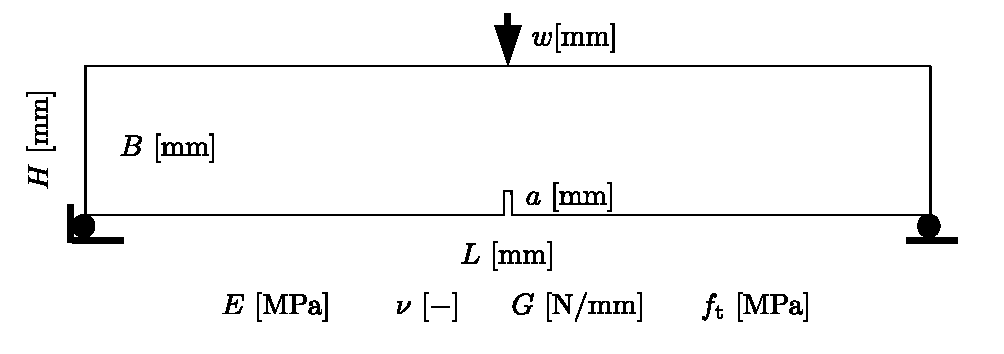
\includegraphics[width=12cm]{fig/Lecture09/figure_bending}
\caption{Geometry and boundary donditions of the three-point bending test.}
\label{FIGf_bending}
\end{figure}

\begin{bmcsex}{Regularized numerical model of a bending test}{ex91_bending_test}
The finite element discretization in this model applies the symmetry condition at the middle section of the beam.  
Upon loading loading, the damage will localize at the tip of the notch and propagate upwards.
This process with simultaneous evaluation of the energy dissipation is provided in the BMCS application 
\texttt{Tensile test - isotropic damage}.

\paragraph{Tasks}
\begin{itemize}
\item Change the size of the softening zone to half and double size. Check to see if you get mesh-independent results.
\item Vary the value of fracture energy $G_f$ - how does it affect the test response?
\item Compare the total amount of dissipated energy $G$ at the end of the loading with nearly zero force with the input value of the damage function $G_\mathrm{F}$. How are they related?
\item Vary the size of the notch and evaluate the amount of dissipated energy. Could a test without a notch be used to obtain a realistic estimate of fracture energy $G_\mathrm{F}$?
\end{itemize}
\end{bmcsex}

\begin{figure}
\centering
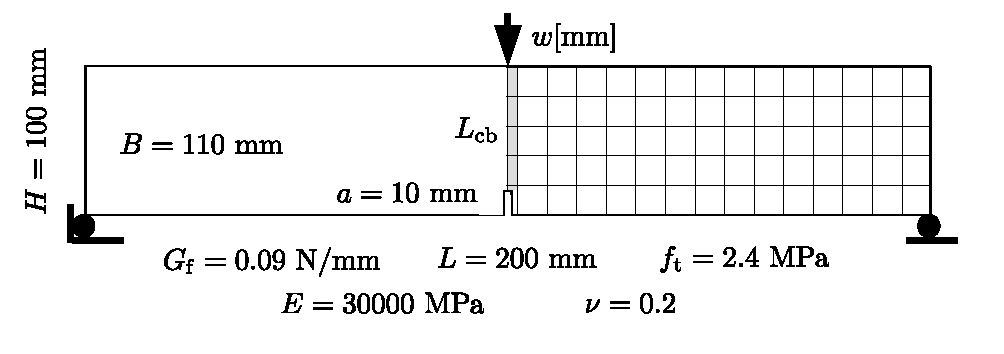
\includegraphics[width=12cm]{fig/Lecture09/figure_fe}
\caption{Finite element disretization used for the verification of mesh-independency of the numerical model.}
\label{FIGf_bending}
\end{figure}

\paragraph{Direct evaluation of the fracture energy:}
Recalling that we can characterize the stable process of crack propagation by an amount of energy needed to produce a unit crack area, i.e. fracture energy $G_\mathrm{F}$, we can choose a more efficient and pragmatic approach determining the fracture energy directly from the test without having to perform numerical calibration. This is the idea behind the standardized characterization procedure proposed by the RILEM committee. Recall that at the point of failure, the whole energy has been consumed to produce the crack of a surface area $A = b(h-a)$, where $h$ and $b$ denote the height and width of the beam and $a$ is the notch depts. Then assuming uniform dissipation during a stable crack propagation we can set
\begin{align}
G_\mathrm{F}=\frac{W}{b\left(h-a\right)},
\label{EQfracturenergyrilem}
\end{align}
However, this simple approach would ignore the fact that self-weight of the beam also invoked some deflection $w_0$. Neither the self-weight load, nor the corresponding deflection are included in the experimentally recorded curve. The situation is illustrated in Fig.~\ref{FIGf_gravity}. 
This effect might be relevant for large specimens. A simple remedy has been suggested by Petersson in the form
%
\begin{align}
G_\mathrm{F}=\frac{W_1+mgw_0}{b\left(h-a\right)},
\label{EQfracturenergyrilem}
\end{align}
where  $mg$ is the weight of the beam. Let us now present an application of the model to tests conducted by Petersson. 

\section{Petersen three-point bending test series}

The original test setup for three-point bending test has been introduced by Petersson who conducted a series of stable tensile tests and three-point-bending tests on notched concrete specimens aiming at characterization of fracture properties such as tensile strength and fracture energy. In the bending test series a group of large-span beams with span length of $L=2000\,\mathrm{mm}$, height of $h=200\,\mathrm{mm}$ and width of $b=50\,\mathrm{mm}$ and notch length of $a=100\,\mathrm{mm}$ were tested (Fig.~\ref{FIGpet1}). 
The ratio of the notch length to the depth of the beam $a/h$ is set to 0.5. 
The specimens were loaded at the middle by the vertical force $F$. The vertical displacement of the loading point $w$ was recorded during the test. 

\mnote{Effect of the shape of softening law}
Let us now ask the question, what material parameters do we need to model this type of response using a non-linear finite element code. What parameters do we know in advance and what are still missing? We know the $E$ modulus and the Poisson's modulus $\nu$, but we do not know the strain-softening law that would characterize the concrete matrix, i.e. the process of crack localization within a fracture process zone. 

\paragraph{Direct evaluation of fracture energy:}

Applying this method to the considered series of tests performed by 
Petersson mean value of the fracture energy has been quantified to $G_\mathrm{F} = 0.124\,\mathrm{N/mm}$.  
\begin{figure}
\centering
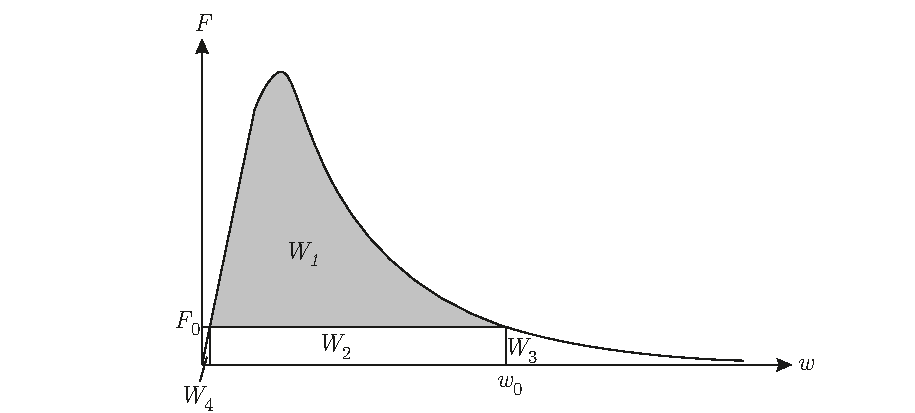
\includegraphics[width=12cm]{fig/F-w-Gf}
\caption{Fracture energy dissipation including the self-weight.}
\label{FIGf_gravity}
\end{figure}
This correction is only approximate and leads to a non-negligible error in case of large specimens. Therefore, weight compensation is also employed in order to achieve a zero reference state for the evaluation of energy supply during the bending test.

\mnote{Iterative calibration of the softening law:}
This situation resembles the case of the calibration of the bond-slip law discussed.
There, we were identifying the parameters of the bond-slip model by iteratively adjusting the damage function and the hardening modulus with the goal to fit the pull-out response of the numerical model with the experiment. 
The same procedure can be applied here to identify the crack localization and propagation characteristics. 
Indeed, we can apply the same concept to identify the softening law $f(w)$ iteratively by adjusting the parameters of its approximation. However, as we have already experienced in case of bond-slip law, this kind of trial-and-error approach is not really efficient. It might be automated using a numerical optimization algorithm that would minimize the lack of fit between the experimental and numerical response curve.

\paragraph{Numerical simulation of Petersson tests}
The simulation  shown in Fig.~\ref{FIGpet1} is done using 4-node bilinear quadrilateral elements. The model is discretized using fine mesh at the mid-span region, where the localization of the strains is expected. To be sure that there is no numerical bias, let us first verify the convergence of the model. Particular attention needs to be paid to the support regions which are susceptible to stress concentration which can distort the results. The applied finite element discretization of the test is shown in Fig.~\ref{FIGpet1}b with fine mesh within the fracture process zone using element size of $10\,\mathrm{mm} \times 10\,\mathrm{mm}$. Material parameters used in the simulation are summarized in Table~\ref{TABpeterssontestsmat}.
%
\paragraph{Simulation results} Fig.~\ref{FIGpet1}c shows plot of damage parameter $\omega$ at mid-span of the beam. Load-point deflection $w$ is plotted versus force $F$ in Fig.~\ref{FIGpet1}d for fracture energy  $G_\mathrm{f}=0.124\,\mathrm{N/mm}$. Petersson also compared the numerical results with the experiments for the range of fracture energy between the lowermost and uppermost obtained values $0.115\,\mathrm{N/mm} \leq G_\mathrm{f} \leq 0.137\,\mathrm{N/mm}$. The same comparison of load-displacement curves is done here using microplane damage model with variation of fraction energy between the given values (Fig.~\ref{FIGpet1}e).
%
\begin{table}\centering
\caption{Material parameter for simulation of Petersson bending test series}
%\renewcommand{\arraystretch}{1.3}% Wider
\begin{tabular}{l ccc}
        \textbf{Description} & \textbf{Symbol} & \textbf{Value} & \textbf{Unit}\\
  \hline
	elasticity modulus & $E$ & $30000$ & $\mathrm{N/mm^2}$ \\
  tensile strength & $f_\mathrm{t}$ & $3.3$ & $\mathrm{N/mm^2}$ \\
  fracture energy & $G_\mathrm{f}$ & $0.124$ & $\mathrm{N/mm}$ \\
\end{tabular}
\label{TABpeterssontestsmat}
\end{table}

\paragraph{Choice of the softening law:}
With the determined amount of the fracture energy $G_\mathrm{F}$ we still do not know the shape of the softening law. 
Similarly to the previous cases, additional simplifying assumptions on the shape of the softening law need to be made.
An example of such an assumption is provided by the exponential cohesive law \ref{eq:fracture_based_cohesive_law} 
derived previously in Chapter \ref{LEC:CohesiveZone}. 

Last question to be addressed is how can we implement the strain softening law into the finite element code? How to ensure objectivity of results and avoid the mesh bias? Example studies performed in Abaqus.

\begin{figure}
\centering
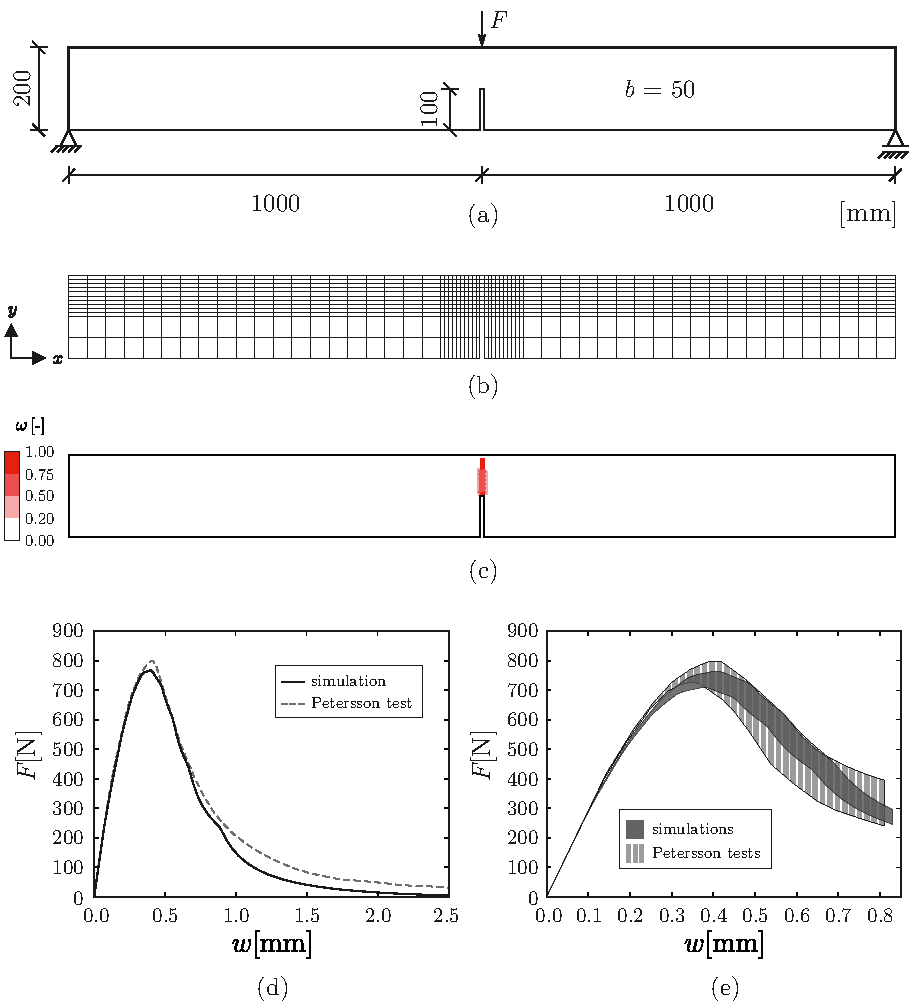
\includegraphics[width=13cm]{fig/3pb-pet.pdf}
\caption{(a) Dimensions of notched three-point-bending test series by Petersson, loading and boundary condition; (b) finite element descritization; (c) damage propagation; (d) load-displacement curves from test and simulations with fracture energy $G_\mathrm{f} = 124\,\mathrm{N/mm}$; (e) range of load-displacement curves from test and simulations with variation of fracture energy $0.115\,\mathrm{N/mm} \leq G_\mathrm{f} \leq 0.137\,\mathrm{N/mm}$}
\label{FIGpet1}
\end{figure}

\section{Onset of damage}
\label{sec:equivalent_strain}
The shown examples are two-dimensional. They describe the strain state and stress state using tensors. 
But the damage function used so far was based on a scalar input, either the tensile strain $\varepsilon_{xx}$ or slip $s$. However, in 2D, there are three variables and in 3D six independent variables describing the strain state at a single material point. Therefore, an equivalant scalar strain measure must be defined to introduce the damage model.  
\subsection{Rankine failure surface}
The simplest case of equivalent strain measure is introduced as the maximum value of the principal tensile strain
\begin{equation}\label{eq:rankine_eq}
\tilde{\varepsilon} = \frac{1}{E} \mathrm{max}(\sigma_i), \qquad i=1,2,3  
\end{equation}
The principal stresses are obtained as the eigenvalues of the stress tensor.

\subsection{Mazars failure surface}
Another variant of equivalent yield surface is defined as follows
\begin{equation}\label{eq:mazars_eq}
\tilde{\varepsilon} = ||\langle
{\boldsymbol{\varepsilon}}
\rangle || = \sqrt{\langle \boldsymbol{\varepsilon} \rangle  : \langle \boldsymbol{\varepsilon} \rangle} = \sqrt{ {\langle \varepsilon_1\rangle}^2   + {\langle\varepsilon_2 \rangle}^2 + {\langle\varepsilon_3 \rangle}^2}
\end{equation}
In ~\ref{eq:mazars_eq}, the McAuley brackets $\langle . \rangle$ means the positive part of (.), e.g. $\langle x \rangle = (x+|x|)/2$. And $\varepsilon_1, \varepsilon_2, \varepsilon_3$ are the principal strains.




\end{document}